\subsection{Reaction Wheel Configuration}
\label{ref:reactConfig}

The satellite should be capable of tracking an Earth station in order to be able to downlink data effectively. Tracking a ship requires similar control capability, since the velocity of the wheel is practically zero compared to the velocity of the satellite. Directing the antennas to the nadir continuously only requires keeping a satellite angular velocity equal to the orbit's angular velocity.
Tracking the Earth station requires torque from the actuators, the torque demand can be calculated based on the angular acceleration demand for Earth station tracking.

\todo{move the first paragraph}

Studies have been conducted on what is the best configuration of redundant reaction wheels. The optimal configuration can of course depend on the requirements. If the requirement is to have the same controllability for reaction wheels in case of fault, and 6 reaction wheels are available, orthogonally configured double reaction wheels can be used. Minimizing energy consumption is normally the goal in deciding on a configuration. Ismail et al. \cite{ReactionWheelConfigSim} investigated several configurations by running simulations with the configuration being the only difference. The tetrahedron configuration of 4 reaction wheels has been chosen as the default configuration in the present thesis, which is quite widespread in the field \cite{reactConfigNasa}, and is redundant with an excess of one wheel. The tetrahedron configuration is visualized in Figure \ref{fig:tetrahedron}.
In tetrahedron configuration the 4 wheel orientations are evenly distributed, unlike the also widespread pyramid configuration. 

\begin{figure}[H]
	\centering 
	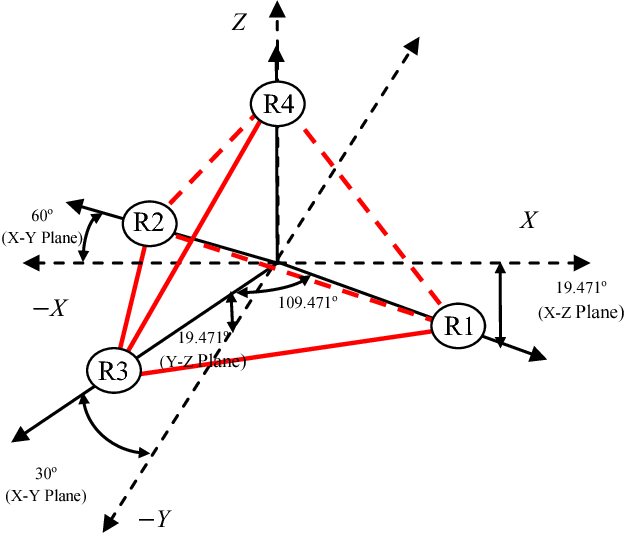
\includegraphics[width=120mm]{figures/tetrahedron}	
	\caption{Geometry of the tetrahedron configuration \cite{Kumar2015DesignAD}}
	\label{fig:tetrahedron}
\end{figure}

%Tetrahedron configuration can output twice as much force along an axis as one wheel can produce along its own axis.
%\cite{reactionWheelConfigThesis} 

\subsubsection{Transformation Between Body \& Reaction Wheel Space}

The main attitude controller sends torque demand signal to the actuators. The reaction wheel torque demand has to be converted from body frame to torques parallel to reaction wheel axes. This transformation is nontrivial. Transforming back from reaction wheel space to body frame is quite intuitive. Knowing the orientation, the mounting angle of each motor axis and the corresponding motor torque, the torque in body frame for tetrahedral configuration can be derived according to equation \ref{eq:motorTrans1} - \ref{eq:transmatrix}. The matrix for tetrahedron configuration is given by \cite{reactionWheelConfigThesis}.

\begin{equation}
\label{eq:motorTrans1}
\vec{N_{rw}} = \underline{A}_{M} \vec{N_{M}} = \begin{bmatrix}
\vec{Axis^{M}_{1}}       & \vec{Axis^{M}_{2}}   & \vec{Axis^{M}_{3}}   & \vec{Axis^{M}_{4}} 
\end{bmatrix} \vec{N_{M}}
\end{equation}

\begin{equation}
\underline{A}_{M} \vec{N_{M}}  = 
\begin{bmatrix}
\cos(19.47)       & -\cos(19.47) \cos(60)  &  -\cos(19.47) \cos(60)  & 0 \\
0       & \cos(19.47) \cos(30)  &  -\cos(19.47) \cos(30)  & 0 \\
-\sin(19.47)       & -\sin(19.47)   &  -\sin(19.47)   & 1
\end{bmatrix} \vec{N_{M}}
\label{eq:transmatrix}
\end{equation}

where $\vec{N_{rw}}$ is the reaction wheel torque in body frame, $\vec{N_{M}}$ is the vector containing the reaction wheel DC motor torques parallel to their axes, $\vec{Axis^{M}_{i}}$ are the reaction wheel motor orientation in body frame, $\underline{A}_{M}$ is the transformation matrix between axis oriented reaction wheel torque and torques in 3 dimensional body frame.

The transformation matrix for orthogonal configuration is quite trivial, and is presented in equation \ref{eq:orthoMatrix}.

\begin{equation}
\underline{A}_{M,orth}  = 
\begin{bmatrix}
1       & 0  &  0 \\
0       & 1  &  0  \\
0       & 0   & 1
\end{bmatrix} 
\label{eq:orthoMatrix}
\end{equation}


\nomenclature[S]{$\vec{N_{rw}}$}{Reaction wheel torque in body frame }
\nomenclature[S]{$\vec{N_{M}}$}{$4\times1$ vector containing the reaction wheel motor motor torques parallel to their axes }
\nomenclature[SAdc]{$\underline{A}_{M}$}{Transformation matrix between axis oriented reaction wheel torque and torques in 3 dimensional body frame }

The nontrivial body frame to motor frame transformation can be derived by reordering equation  \ref{eq:motorTrans1}. Since $\underline{A}_{M} $ is a $ 4 \times 3 $ matrix, a pseudo inverse has to be used when reordering the equation, as presented in equation \ref{eq:motorTrans}. 

\begin{equation}
\label{eq:motorTrans}
\vec{N_{M}} =  \underline{A}_{M} ^\dagger \vec{N_{rw}}   =  \underline{A}_{M}^T  (\underline{A}_{M} \underline{A}_{M} ^T)^{-1} \vec{N_{rw}}
\end{equation}

\begin{figure}[H]
	\centering 
	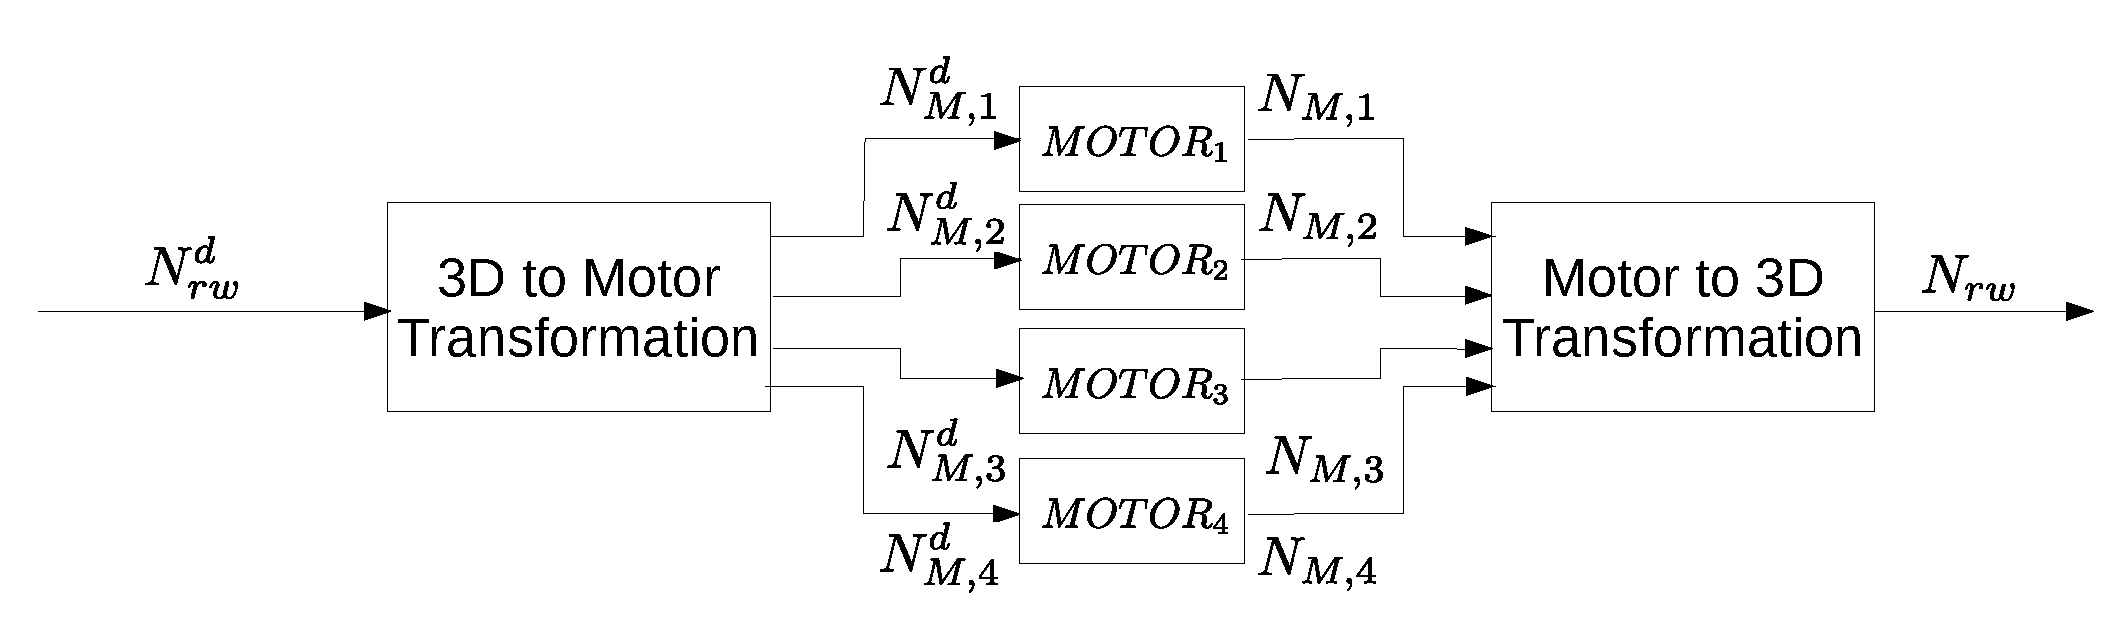
\includegraphics[width=170mm]{figures/distribution}	
	\caption{Reaction wheel torque distribution}
	\label{fig:torqueDistribution}
\end{figure}


%\begin{equation}
%h_{rot} = A\left[ h_1, h_2, h_3, h_4 \right]^T
%\end{equation}

In case there's a demand to adjust the torque distribution between the wheels, an extra vector can be included, as shown in equation \ref{eq:TorqueDistrib}
\cite[equation 18.41-42]{SADC}. If k is set to 0, the norm of wheel torques are minimized.

\begin{equation}
\label{eq:TorqueDistrib}
 \vec{N_{M}} = \underline{A}^\dagger_{M} \vec{N_{rw}}  + k\left[1,-1,-1,1\right]^T
\end{equation}


